\documentclass{report}

\usepackage{float}
\usepackage{pgfplots}
\usepackage[top=2cm,left=2cm,right=2cm,bottom=2cm]{geometry}

\title{Electromagnetic Labs}
\author{Shawal Mbalire \\21/U/0851 \\BELE}

\begin{document}
    \maketitle


    \begin{table}[H]
        \centering
        \begin{tabular}{cc}
        \hline
        Length(mm) & Column 2 \\
        \hline
        0.00 & 0.113 \\
        0.01 & 0.144 \\
        0.02 & 0.187 \\
        0.03 & 0.231 \\
        0.04 & 0.279 \\
        0.05 & 0.312 \\
        0.06 & 0.349 \\
        0.07 & 0.416 \\
        0.08 & 0.471 \\
        0.09 & 0.516 \\
        0.10 & 0.574 \\
        0.11 & 0.631 \\
        0.12 & 0.684 \\
        0.13 & 0.721 \\
        0.14 & 0.746 \\
        0.15 & 0.736 \\
        0.16 & 0.601 \\
        0.17 & 0.195 \\
        0.18 & 0.119 \\
        0.19 & 0.139 \\
        0.20 & 0.176 \\
        0.21 & 0.207 \\
        0.22 & 0.250 \\
        0.23 & 0.287 \\
        0.24 & 0.326 \\
        0.25 & 0.380 \\
        0.26 & 0.434 \\
        0.27 & 0.512 \\
        0.28 & 0.567 \\
        0.29 & 0.620 \\
        0.30 & 0.683 \\
        0.31 & 0.731 \\
        0.32 & 0.739 \\
        0.33 & 0.741 \\
        0.34 & 0.650 \\
        0.35 & 0.263 \\
        0.36 & 0.122 \\
        0.37 & 0.123 \\
        0.38 & 0.164 \\
        0.39 & 0.205 \\
        0.40 & 0.237 \\
        \hline
        \end{tabular}
        \caption{}
    \end{table}


    \begin{figure}[H]
        \centering
        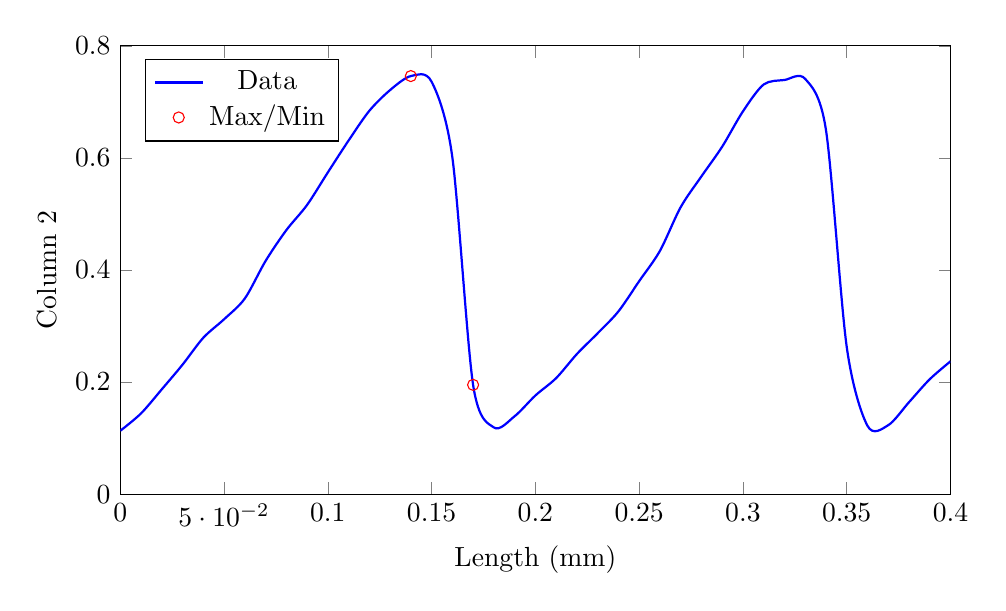
\begin{tikzpicture}
        \begin{axis}[
          width=\linewidth,
          height=0.6\linewidth,
          xmin=0, xmax=0.40,
          ymin=0, ymax=0.8,
          xlabel=Length (mm),
          ylabel=Column 2,
          legend pos=north west
        ]
        
        \addplot [smooth, thick, blue] table {
        0.00 0.113
        0.01 0.144
        0.02 0.187
        0.03 0.231
        0.04 0.279
        0.05 0.312
        0.06 0.349
        0.07 0.416
        0.08 0.471
        0.09 0.516
        0.10 0.574
        0.11 0.631
        0.12 0.684
        0.13 0.721
        0.14 0.746
        0.15 0.736
        0.16 0.601
        0.17 0.195
        0.18 0.119
        0.19 0.139
        0.20 0.176
        0.21 0.207
        0.22 0.250
        0.23 0.287
        0.24 0.326
        0.25 0.380
        0.26 0.434
        0.27 0.512
        0.28 0.567
        0.29 0.620
        0.30 0.683
        0.31 0.731
        0.32 0.739
        0.33 0.741
        0.34 0.650
        0.35 0.263
        0.36 0.122
        0.37 0.123
        0.38 0.164
        0.39 0.205
        0.40 0.237
        };
        
        \addplot [only marks, mark=o, red] coordinates {
        (0.14,0.746) % maximum point
        (0.17,0.195) % minimum point
        };
        
        \legend{Data,Max/Min}
        \end{axis}
        \end{tikzpicture}
    \end{figure}


    \begin{table}[H]
        \centering
        \begin{tabular}{cc}
        \hline
        Length(mm) & Column 2 \\
        \hline
        0.00 & 0.757 \\
        0.01 & 0.770 \\
        0.02 & 0.786 \\
        0.03 & 0.797 \\
        0.04 & 0.794 \\
        0.05 & 0.784 \\
        0.06 & 0.760 \\
        0.07 & 0.737 \\
        0.08 & 0.703 \\
        0.09 & 0.642 \\
        0.10 & 0.611 \\
        0.11 & 0.568 \\
        0.12 & 0.552 \\
        0.13 & 0.559 \\
        0.14 & 0.578 \\
        0.15 & 0.608 \\
        0.16 & 0.655 \\
        0.17 & 0.693 \\
        0.18 & 0.730 \\
        0.19 & 0.769 \\
        0.20 & 0.780 \\
        0.21 & 0.796 \\
        0.22 & 0.799 \\
        0.23 & 0.791 \\
        0.24 & 0.771 \\
        0.25 & 0.738 \\
        0.26 & 0.701 \\
        0.27 & 0.668 \\
        0.28 & 0.619 \\
        0.29 & 0.572 \\
        0.30 & 0.550 \\
        0.31 & 0.548 \\
        0.32 & 0.564 \\
        0.33 & 0.595 \\
        0.34 & 0.639 \\
        0.35 & 0.671 \\
        0.36 & 0.708 \\
        0.37 & 0.742 \\
        0.38 & 0.770 \\
        0.39 & 0.784 \\
        0.40 & 0.794 \\
        \hline
        \end{tabular}
        \caption{6dB attenuator}
    \end{table}


    \begin{figure}[H]
        \centering
        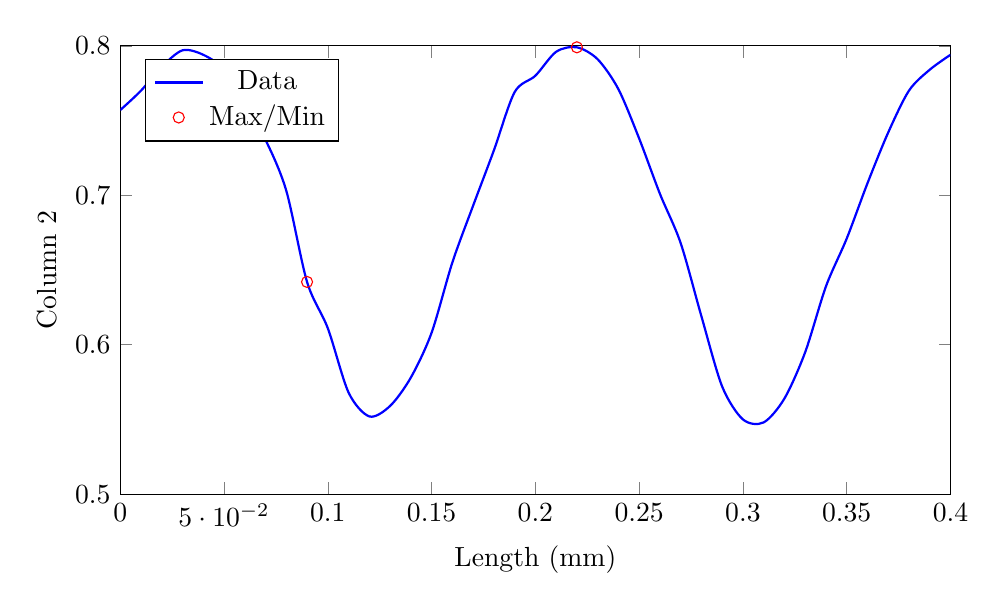
\begin{tikzpicture}
        \begin{axis}[
        width=\linewidth,
        height=0.6\linewidth,
        xmin=0, xmax=0.40,
        ymin=0.5, ymax=0.8,
        xlabel=Length (mm),
        ylabel=Column 2,
        legend pos=north west
        ]
        
        \addplot [smooth, thick, blue] table {
        0.00 0.757
        0.01 0.770
        0.02 0.786
        0.03 0.797
        0.04 0.794
        0.05 0.784
        0.06 0.760
        0.07 0.737
        0.08 0.703
        0.09 0.642
        0.10 0.611
        0.11 0.568
        0.12 0.552
        0.13 0.559
        0.14 0.578
        0.15 0.608
        0.16 0.655
        0.17 0.693
        0.18 0.730
        0.19 0.769
        0.20 0.780
        0.21 0.796
        0.22 0.799
        0.23 0.791
        0.24 0.771
        0.25 0.738
        0.26 0.701
        0.27 0.668
        0.28 0.619
        0.29 0.572
        0.30 0.550
        0.31 0.548
        0.32 0.564
        0.33 0.595
        0.34 0.639
        0.35 0.671
        0.36 0.708
        0.37 0.742
        0.38 0.770
        0.39 0.784
        0.40 0.794
        };
        
        \addplot [only marks, mark=o, red] coordinates {
        (0.22,0.799) % maximum point
        (0.09,0.642) % minimum point
        };
        
        \legend{Data,Max/Min}
        \end{axis}
        \end{tikzpicture}
    \end{figure}
    

    \begin{table}[H]
        \centering
        \begin{tabular}{cc}
        \hline
        Length(mm) & Column 2 \\
        \hline
        0.00 & 0.752 \\
        0.01 & 0.750 \\
        0.02 & 0.742 \\
        0.03 & 0.735 \\
        0.04 & 0.721 \\
        0.05 & 0.692 \\
        0.06 & 0.674 \\
        0.07 & 0.647 \\
        0.08 & 0.629 \\
        0.09 & 0.610 \\
        0.10 & 0.598 \\
        0.11 & 0.598 \\
        0.12 & 0.613 \\
        0.13 & 0.614 \\
        0.14 & 0.634 \\
        0.15 & 0.655 \\
        0.16 & 0.673 \\
        0.17 & 0.698 \\
        0.18 & 0.724 \\
        0.19 & 0.743 \\
        0.20 & 0.751 \\
        0.21 & 0.742 \\
        0.22 & 0.730 \\
        0.23 & 0.715 \\
        0.24 & 0.685 \\
        0.25 & 0.666 \\
        0.26 & 0.640 \\
        0.27 & 0.625 \\
        0.28 & 0.606 \\
        0.29 & 0.601 \\
        0.30 & 0.601 \\
        0.31 & 0.607 \\
        0.32 & 0.623 \\
        0.33 & 0.642 \\
        0.34 & 0.668 \\
        0.35 & 0.697 \\
        0.36 & 0.718 \\
        0.37 & 0.734 \\
        0.38 & 0.744 \\
        0.39 & 0.744 \\
        0.40 & 0.738 \\
        \hline
        \end{tabular}
        \caption{Termination load}
    \end{table}


    \begin{figure}[H]
        \centering
        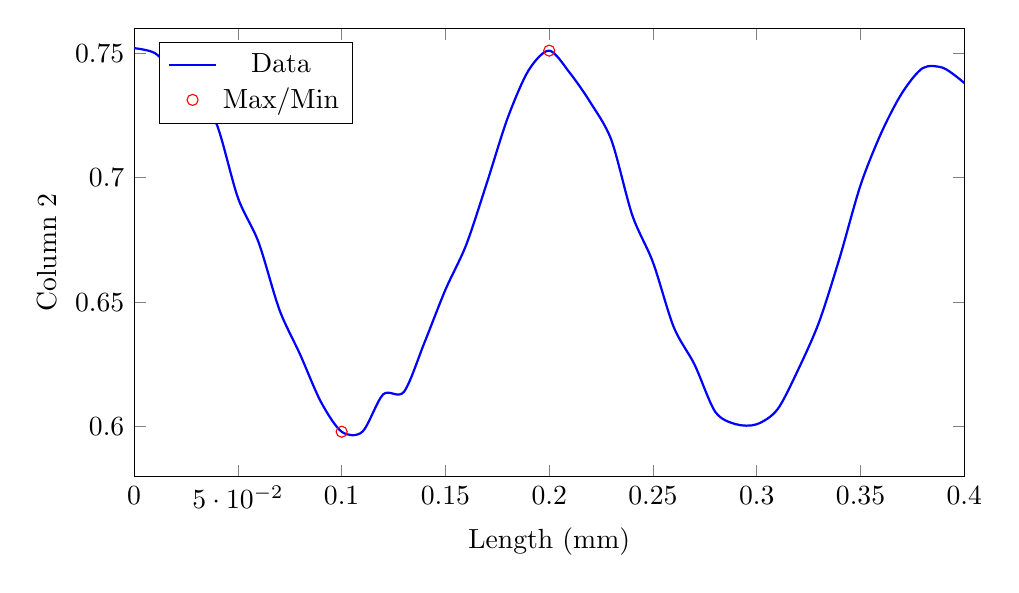
\begin{tikzpicture}
        \begin{axis}[
          width=\linewidth,
          height=0.6\linewidth,
          xmin=0, xmax=0.40,
          ymin=0.58, ymax=0.76,
          xlabel=Length (mm),
          ylabel=Column 2,
          legend pos=north west
        ]
        
        \addplot [smooth, thick, blue] table {
        0.00 0.752
        0.01 0.750
        0.02 0.742
        0.03 0.735
        0.04 0.721
        0.05 0.692
        0.06 0.674
        0.07 0.647
        0.08 0.629
        0.09 0.610
        0.10 0.598
        0.11 0.598
        0.12 0.613
        0.13 0.614
        0.14 0.634
        0.15 0.655
        0.16 0.673
        0.17 0.698
        0.18 0.724
        0.19 0.743
        0.20 0.751
        0.21 0.742
        0.22 0.730
        0.23 0.715
        0.24 0.685
        0.25 0.666
        0.26 0.640
        0.27 0.625
        0.28 0.606
        0.29 0.601
        0.30 0.601
        0.31 0.607
        0.32 0.623
        0.33 0.642
        0.34 0.668
        0.35 0.697
        0.36 0.718
        0.37 0.734
        0.38 0.744
        0.39 0.744
        0.40 0.738
        };
        
        \addplot [only marks, mark=o, red] coordinates {
        (0.20,0.751) % maximum point
        (0.10,0.598) % minimum point
        };
        
        \legend{Data,Max/Min}
        \end{axis}
        \end{tikzpicture}
    \end{figure}

\end{document}